\subsection{Quadratische Funktionen}
Nach den linearen sind die sogenannten quadratischen Funktionen noch relativ einfach. Sie werden auch als Parabelgleichungen bezeichnet. Ihren Namen verdanken diese Funktionen der Tatsache, dass ihre Variable zumindest einmal quadratisch und niemals mit einem h"oheren Exponenten als $2$ in die Funktion mit eingeht.\\
Um diese Definition jedoch richtig zu verstehen, m"ussen wir zun"achst einmal anschauen, was ein Exponent ist:

\subsection{Exponent und Basis}
Die Worte Exponent und Basis, spielen immer dann eine Rolle in der Mathematik, wenn es sich um ein Konstrukt wie $a^b$ handelt (Gesprochen: "'a hoch b"').\\
In diesem Konstrukt wird "'a"' als Basis und "'b"' als Exponent bezeichnet. Hierbei gilt:
\begin{itemize}
	\item $a^0 = 1$
	\item $a^1 = a$
	\item $a^2 = a \cdot a$
	\item $a^3 = a \cdot a \cdot a$
	\item $a^4 = a \cdot a \cdot a \cdot a$
	\item $\ldots$
\end{itemize}

\paragraph{Rechengesetze f"ur Exponenten}
\begin{enumerate}
	\item $((b)^n)^m = b^{n \cdot m}$
	\item $b^n \cdot b^m = b^{n+m}$
	\item $\frac{b^n}{b^m} = b^{n-m}$
\end{enumerate}

\noindent Will man nun, solch eine Funktion umkehren, so muss man die n-te Wurzel ziehen:
\paragraph{Beispiel f"ur Wurzeln}
\begin{enumerate}
	\item $f(x)=x^2 => f^{-1}(y)=\sqrt[2]{y}$ oder k"urzer $f^{-1}(y)=\sqrt{y}$
	\item $f(x)=x^3 => f^{-1}(y)=\sqrt[3]{y}$
	\item $f(x)=x^4 => f^{-1}(y)=\sqrt[4]{y}$
\end{enumerate}

\paragraph{Rechengesetze f"ur Wurzeln}
\begin{enumerate}
	\item $\sqrt[m]{a} = a^{\frac{1}{m}}$
	\item $\sqrt[m]{a} \cdot \sqrt[m]{b} = \sqrt[m]{a \cdot b}$
	\item $\frac{\sqrt[m]{a}}{\sqrt[m]{b}} = \sqrt[m]{\frac{a}{b}}$
	\item $\sqrt[m]{b^n} = b^{\frac{n}{m}}$
\end{enumerate}\vline

\noindent Im Fall $a^2$ wird auch oft einfach nur "'a zum Quadrat"' gesagt.\\
Dies kommt daher, dass ein Quadrat aus vier gleich langen Seiten besteht und es sich bei allen Innenwinkel (die Winkel innerhalb des Rechtecks), um so genannte "'rechte Winkel"' (genau 90 Grad) handelt. Die Fläche eines Quadrats, mit der Seitenl"ange a, l"asst sich deshalb mit der Formel $a \cdot a$ oder auch $a^2$ berechnen.

\subsubsection{Die Normalparabel}
Die Normalparabel besitzt die Formel 
\begin{equation*}
f(x) = x^2
\end{equation*}
Sie ist eine nach oben ge"offnete, achsensymmetrische Kurve dar, deren niedrigster Punkt (Scheitel) $S$ im Ursprung des Koordinatensystems $(0,0)$ liegt.

%Siehe: Verschieben einer Funktion
%\subsubsection{Verschieben einer Parabel}
%Wollen wir eine 
%Eine Parabel l"asst sich um den Wert $x_s$ in $x$-Richtung verschieben, indem man diesen Wert von der Variable $x$ subtrahiert, daraus folgt:\\
%$f(x)=(x-x_s)^2$\vspace{0.25 cm}\flushleft
%Durch Addition des gesamten Terms mit dem Wert $y_s$ wird die Parabel um den gleichen Wert in y-Richtung verschoben.\\
%Die Gleichung der Parabel lautet nun wie folgt:\\
%$f(x)=(x-x_s)^2+y_s$\\
%Ihr Scheitel besitzt die Koordinaten $S(x_s,y_s)$.

\subsubsection{Stauchen und Strecken}
Durch Multiplizieren der Normalparabel mit einer konstanten $a$ l"asst sich die Kurve stauchen oder strecken $f(x)=a \cdot x^2$. Ist der Betrag von $a$ kleiner $1$, so wird die Parabel gestaucht (siehe Abb. \ref{fig:parabel}). Ist er gr"o"ser $1$, so wird sie gestreckt. Dar"uber hinaus wird die Funktion durch einen negativen Wert von a an der $x$-Achse gespiegelt und die Parabel ist somit nach unten ge"offnet.
\begin{figure}[h!]
\begin{center}
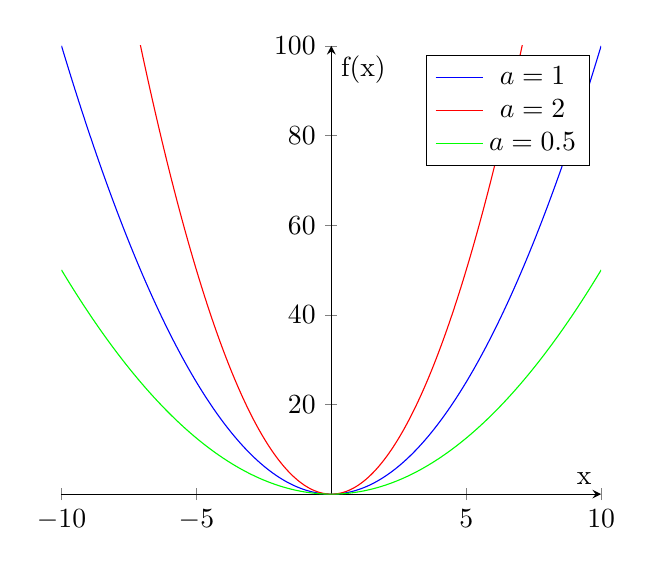
\begin{tikzpicture}[scale = 1.0]
    \begin{axis}[
        domain=-10:10,
        xmin=-10, xmax=10,
        ymin=-0, ymax=100,
        samples=400,
        axis y line=center,
        axis x line=middle,
        xlabel={x},
        ylabel={f(x)},
    ]
    	  \addlegendentry{$a=1$}
    	   \addplot+[mark=none, color=blue] {x*x};
    	   \addlegendentry{$a=2$}
       \addplot+[mark=none, color=red] {2 * x*x};
       \addlegendentry{$a=0.5$}
       \addplot+[mark=none, color=green] {0.5 * x*x};
    \end{axis}
\end{tikzpicture}
\end{center}
\caption{Normalparabel (blau), gestreckte (rot) und gestauchte Normalparabel (gr"un).}
\label{fig:parabel}
\end{figure}

\subsubsection{Die Scheitelform}
Durch Kombination von Stauchung/Streckung und Verschiebung erh"alt man die so genannte Scheitelform: 
\begin{equation*}
f(x)=a(x-x_s)^2+y_s.
\end{equation*}
Mithilfe dieser Form lassen sich alle Arten quadratischer Funktionen darstellen. Au"serdem lassen sich die Koordinaten des Scheitels, der Stauchungs- bzw. Streckungsfaktor der Funktion, sowie die Frage, ob sie nach oben oder unten ge"offnet ist, auf einfachste Weise bestimmen.

\subsubsection{Die Normalform einer quadratischen Gleichung}
Multipliziert man die Scheitelform aus, so erh"alt man 
\begin{equation*}
f(x)=a \cdot x^2-2 \cdot a \cdot x_sx+x_s^2+y_s.
\end{equation*}
Ersetzt man nun die konstanten Werte $-2ax_s$ durch $b$ und $x_s^2+y_s$ durch $c$, so erh"alt man die \textbf{Normalform} quadratischer Gleichungen:
\begin{equation*}
f(x)=a \cdot x^2+b \cdot x+c
\end{equation*}

\subsubsection{Verschieben einer Funktion (f"ur alle Funktionen)} \label{sec:verschieben}
Angenommen wir haben eine Funktion $f$ mit $\mathbb{D} = \mathbb{R}$ und wollen eine neue Funktion $f^*$ bauen, wobei wir diese um $d > 0$ nach rechts verschieben wollen. Damit muss gelten:
\begin{equation*}
\forall x \in \mathbb{R} :  f^*(x) = f(x-d) \iff \forall x \in \mathbb{R} : f^*(x+d) = f(x).
\end{equation*}
Wir nehmen also einfach die gegebene Funktion $f(x)$ und ersetzen jedes $x$ durch $x-d$. Setzen wir hingegen $f^*(x) = f(x) + d$ so verschieben wir die Funktion nach oben. F"ur $d < 0$ folgt, dass wir die Funktion nach links bzw. nach unten verschieben.

\subsubsection{Die binomischen Formeln}
Die binomischen Formeln sind das Ergebnis des Ausmultiplizierens, hat man sie jedoch im Kopf so spart man viel Zeit:
\begin{enumerate}
\item $(a+b)^2=a^2+2ab+b^2$
\item $(a-b)^2=a^2-2ab+b^2$
\item $(a+b)(a-b)=a^2-b^2$
\end{enumerate}

\subsubsection{Die quadratische Erg"anzung}
Die quadratische Erg"anzung hilft uns bei der Umwandlung der Normalform in die Scheitelform und somit bei der Bestimmung des Scheitels. Wir werden diese an anhand eines Beispiels erkl"aren.

\paragraph{Beispiel:}
Sei 
\begin{equation*}
f(x) = 3x^2 - 6x - 24.
\end{equation*}
Im ersten Schritt klammern wir die Konstante "'$a$"' (hier gleich $3$) aus:
\begin{equation*}
f(x) = 3x^2 - 6x - 24= 3 \cdot (x^2-2x-8).
\end{equation*}
Schaut man sich nun den Term innerhalb der runden Klammern genauer an, so kann man eine gewisse "Ahnlichkeit mit der ersten, bzw. zweiten binomischen Formel feststellen. Deshalb folgt nun auch der wichtigste Schritt, die eigentliche quadratische Erg"anzung. Wir erg"anzen die Formel nun so, dass wir eine der beiden binomischen Formeln anwenden k"onnen. Daf"ur m"ussen wir erst einmal feststellen, was der $a$- und was der $b$-Wert der binomischen Formeln ist. Die zweite binomische Formel lautet 
\begin{equation*}
(a-b)^2=a^2-2ab+b^2.
\end{equation*}
Vergleichen wir dies mit unserem Term 
\begin{equation*}
x^2-2x-8
\end{equation*}
so sehen wir gleich, dass
\begin{equation*}
a := x \Rightarrow 2ab = 2x \Rightarrow b = 1.
\end{equation*}
Allerdings ist $b^2$ f"ur $b = +1$ nicht $-8$ sondern $1$. Um $f$ nicht zu ver"andern m"ussen wir deshalb eine Korrektur vornehmen:
\begin{equation*}
f(x) = 3 \cdot \left(  \underbrace{(x-1)^2}_{\text{wegen 2. bin. Formel}} + \underbrace{-1^2 - 8}_{\text{da } b^2 = 1 \text{ und nicht } -8 } \right)
\end{equation*}
Hier nochmal die "Ubersicht:
\begin{equation*}
f(x) = 3 \cdot \left(  \underbrace{x^2}_{:=a^2} \underbrace{- 2 \cdot x \cdot 1}_{:= -2ab} \underbrace{+ 1^2}_{:= + b^2} \underbrace{- 1^2 -8}_{:=-\text{Korrektur}} \right)
\end{equation*} 
Nun k"onnen wir noch ein wenig zusammenfassen
\begin{equation*}
f(x) = 3 \cdot ((x-1)^2-1^2-8) = 3((x-1)^2-9) = 3(x-1)^2-27
\end{equation*}
Und voil\`a, schon ist man fertig.

\subsubsection{Berechnung der Nullstellen} \label{sec:quadnullstellen}
Eine Nullstelle ist ein Punkt, an dem der Graph die $x$-Achse schneidet. Anders ausgedr"uckt: Ein Punkt an dem die Funktion $f(x)$ den Wert $0$ erreicht. Um Nullstellen zu berechnen, l"ost man die Gleichung
\begin{equation*}
f(x) = 0,
\end{equation*}
nach $x$. Beispiel: $f(x)=x^2-1$, Nullstellen: $x^2-1=0\implies x^2=1$, L"osungen sind $+1$ und $-1$. Die Gleichung kann also auch mehrere L"osungen haben.\\
Um die Nullstellen von quadratischen Gleichungen zu berechnen, gibt es mehrere M"oglichkeiten.

\paragraph{Zerlegung in Linearfaktoren (auch f"ur Polynome h"oherer Ordnung):}
%\begin{center}
%"'Null multipliziert mit irgendwas ist immer Null"'
%\end{center} % Bitte entfernen. Unendlich mal Null ist undefiniert, und gerade bei Grenzwerten schwierig...

Mit der Linearfaktorzerlegung erhalten wir eine Form der Funktion, die uns sagt f"ur welche $x$ ein Faktor Null und somit die gesamte Funktion Null ergibt. Auch dies zeigen wir an einem Beispiel.

\paragraph{Beispiel}
Sei
\begin{equation*}
f(x) = 6x^2 - 24
\end{equation*}
Wir fragen uns f"ur welche $x$ ist $f(x) = 0$.
\begin{equation*}
f(x) = 0 \iff 6x^2 - 24 = 0 \iff x^2 - 4 = 0 \stackrel{\text{3. bin. Formel}}{\iff} (x-2)(x+2) = 0 
\end{equation*}
Die Faktoren der Funktion sind somit $(x-2)$ und $(x+2)$. $(x-2) = 0$ f"ur $x = 2$ und $(x+2) = 0$ f"ur  $x = -2$. Damit sind die Nullstellen:
\begin{equation*}
N_1 = (2, f(2)) = (2, 0) \text{ und } N_2 = (-2, f(-2)) = (-2, 0)
\end{equation*}

% Was hier folgt ist unsinnig!
%Wenn wir also rein theoretisch die Funktion umkehren und 0 einsetzen, so m"ussten wir die x-Werte der Nullstellen herausbekommen. Wollen wir jedoch eine quadratische Gleichung umkehren, so sto"sen wir allerdings auf ein kleines Problem... \vspace{0.5 cm}\\
%Schauen wir uns daf"ur mal ein Beispiel an:\\
%$y = $\\
%Zun"achst m"usste man daf"ur sorgen, dass das x nicht mehr in zwei verschiedenen Potenzen auftaucht. Dies geht ganz leicht "uber die quadratische Erg"anzung.\\
%$y = 3(x + 0,5)^2 + 3,25 | -3,25\leftrightarrow$\\
%$3(x+0,5)^2 = y-3,25 | :3 \leftrightarrow$\\
%$(x+0,5)^2 = \frac{y-3,25}{3}$\\
%Nun m"ussten wir die Wurzel ziehen. Hier kommt das Problem zum Vorschein.\\
%Die Wurzel einer bestimmten Zahl kann sowohl positiv als auch negativ sein.\\
%Nehmen wir zum Beispiel die Zahl 4: ihre Wurzel ist $\pm 2$.\\
%Da die Regel, dass jedem x-Wert genau ein y-Wert zugeordnet wird, nicht mehr erf"ullt wird, handelt es sich nicht mehr um eine Funktion, sondern um eine Relation.
%Aus diesem Grund gilt auch f"ur unsere Gleichung:\\
%$x+0,5 =\pm \sqrt{\frac{y-3,25}{3}}\leftrightarrow$\\
%$x=0,5 \pm \sqrt{\frac{y-3,25}{3}}$\\
%Nun muss man noch f"ur y  0 einsetzen und gucken was passiert.\\
%In unserem Fall bemerkt man schnell, dass unter der Wurzel ein negativer Wert heraus kommt. Dies darf jedoch nicht sein, da in den reellen Zahlen die Wurzel von negativen Zahlen nicht definiert ist.\\
%Somit hat unsere Funktion keinerlei Nullstellen.

\paragraph{Die L"osungsformel f"ur quadratische Gleichungen (Mitternachtsformel):}
Eine weitere M"oglichkeit, die Nullstellen einer quadratischen Funktion zu berechnen, w"are durch Verwendung der so genannten "'Mitternachtsformel"':
\begin{equation*}
0 = ax^2 + bx + c \Rightarrow x_{1,2} := \frac{-b \pm \sqrt{b^2 - 4ac}}{2a}
\end{equation*}
Falls jedoch 
\begin{equation*}
b^2 - 4ac < 0
\end{equation*}
existiert \textbf{keine Nullstelle}, da wir in den reellen Zahlen keine negative Wurzel kennen und falls
\begin{equation*}
b^2 - 4ac = 0
\end{equation*}
handelt es sich um eine sog. \textbf{doppelte Nullstelle}. Ansonsten handelt es sich um \textbf{zwei Nullstellen}. Dabei nennen wir $b^2 - 4ac$ die Diskriminante.
%Wie man sieht, ist es sehr umst"andlich, jedes Mal die Umkehrrelation zu berechnen und in diese dann f"ur y den Wert 0 einzusetzen... Aus diesem Grund wurden allgemeine Formeln zur Berechnung der Nullstellen quadratischer Gleichungen hergeleitet:\\
%Zun"achst hat man die allgemeine Formel $y = ax^2 + bx +c$ gegeben.\\
%Diese wird "'gleich Null"' gesetzt:\\
%$0 = ax^2 + bx + c$\\
Wie entsteht diese Formel?
\begin{equation*}
 ax^2 + bx + c 
\end{equation*}
Wird auf die Scheitelform gebracht
\begin{equation*}
 ax^2 + bx + c  = \left(x + \frac{b}{2a} \right)^2 - \frac{b^2-4ac}{4a^2}
\end{equation*}
und gleich Null gesetzt
\begin{equation*}
\left(x + \frac{b}{2a}\right)^2 - \frac{b^2-4ac}{4a^2} = 0 \iff x = \frac{-b \pm \sqrt{b^2 - 4ac}}{2a}
\end{equation*}
Den Beinamen "'Mitternachtsformel"' verdankt sie ihrer Wichtigkeit. Sie wird n"amlich tats"achlich so oft gebraucht, dass man sie auch noch auswendig aufsagen k"onnen sollte, wenn man um Mitternacht gefragt wird!% (Auch wenn von euch vermutlich niemand bereits um Mitternacht schl"aft $\ldots$).

\paragraph{Raten der Nullstellen (f"ur alle Funktionen):}
Ist man erfahren genug und die Funktion einfach genug, so kann man h"aufig die Nullstelle auch einfach erraten. Dann muss man noch einen Beweis erbringen, dass es sich wirklich um einen Nullstelle handelt. Hierf"ur setzten wir einfach das geratene $x_0$ in $f(x)$ ein und "uberpr"ufen ob 
\begin{equation*}
f(x_0) \stackrel{?}{=} 0
\end{equation*}


\subsubsection{Symmetrie} \label{sec:symmetrie}
Eine Funktion ist genau dann \textcolor{red}{symmetrisch zur y-Achse}, wenn gilt:
\begin{equation*}
f(x)=f(-x).
\end{equation*}
Solche Funktionen werden auch als \textcolor{red}{gerade} Funktion bezeichnet. Eine Funktion ist genau dann \textcolor{red}{symmetrisch zum Ursprung}, oder auch \textcolor{red}{ungerade}, wenn gilt:
\begin{equation*}
f(-x)=-f(x).
\end{equation*}
Quadratische Funktionen sind immer Achsensymmetrisch, jedoch nicht immer zur y-Achse.
\begin{warning}
	\textbf{\textcolor{red}{Achtung:}} Gerade hat in dem Sinne nichts mit der Geraden zu tun!!!\\
	Die Bezeichnungen gerade und ungerade Funktion stammen daher, dass alle Polynome \ref{polynom}, welche lediglich gerade Exponenten aufweisen, auf jeden Fall symmetrisch sind. Polynome mit ausschließlich ungeraden Exponenten sind Punktsymmetrisch.
\end{warning}
%\begin{description}
%\item[Zwei Nullstellen] Die Funktion besitzt zwei Nullstellen, wenn der Wert der Diskriminante gr"o"ser 0 ist.
%\item[Eine Nullstelle] Die Funktion besitzt nur eine (doppelte) Nullstelle, wenn die Diskriminante 0 ergibt.
%\item[Keine Nullstelle] Die Funktion hat keinerlei Nullstellen, wenn f"ur die Diskriminante ein Wert kleiner 0 heraus kommt.
%\end{description}